\begin{figure}[H]
    \centering
    \caption{Modelo de trânsito procurado pelo método BLS.}
    \label{fig:bls}
    \vspace{-.1cm}
    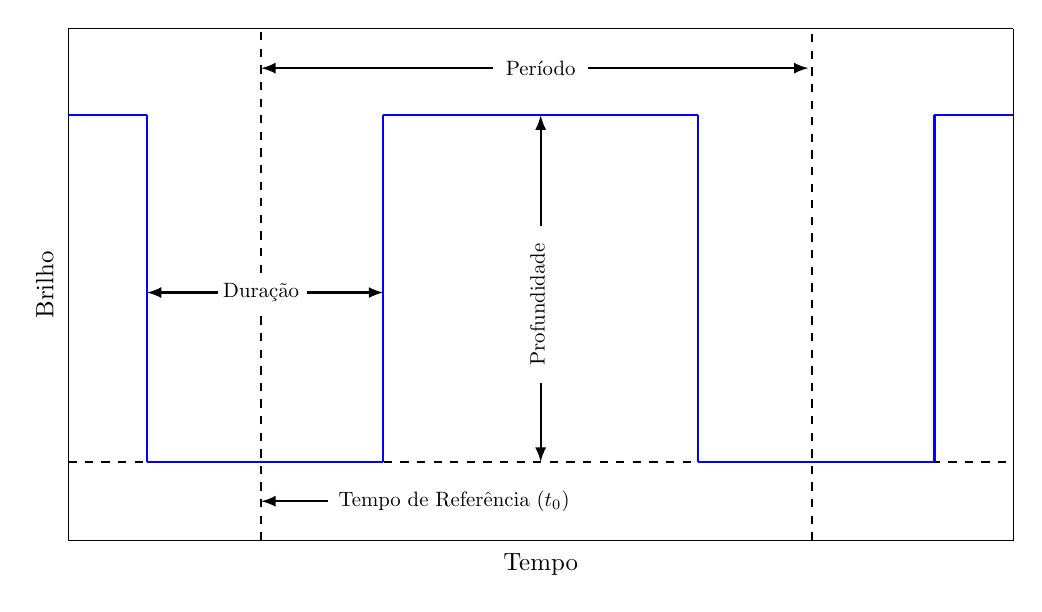
\begin{tikzpicture}
        % Linhas e setas
        \draw [-, color=black, thick, dashed] (0,1)--(12,1);
        
        \draw [-latex, color=black, thick] (6, 2)--(6, 1);
        \draw [-latex, color=black, thick] (6, 4)--(6, 5.4);
        
        \draw [-, color=black, thick, dashed] (2.45,0)--(2.45,2.95);
        \draw [-, color=black, thick, dashed] (2.45,3.4)--(2.45,6.5);
        \draw [-latex, color=black, thick] (1.9, 3.15)--(1, 3.15);
        \draw [-latex, color=black, thick] (3.03, 3.15)--(4, 3.15);
        
        \draw [-, color=black, thick, dashed] (9.45,0)--(9.45,6.5);
        
        \draw [-latex, color=black, thick] (5.4, 6)--(2.45, 6);
        \draw [-latex, color=black, thick] (6.6, 6)--(9.4, 6);
        
        \draw [-latex, color=black, thick] (3.3, 0.5)--(2.45, 0.5);
        
        
        % Gráfico
        \draw [-, color=blue, thick] (0,5.4)--(1,5.4);
        \draw [-, color=blue, thick] (1,5.4)--(1,1);
        \draw [-, color=blue, thick] (1,1)--(4,1);
        \draw [-, color=blue, thick] (4,1)--(4,5.4);
        \draw [-, color=blue, thick] (4,5.4)--(8,5.4);
        \draw [-, color=blue, thick] (8,5.4)--(8,1);
        \draw [-, color=blue, thick] (8,1)--(11,1);
        \draw [-, color=blue, thick] (11,1)--(11,5.4);
        \draw [-, color=blue, thick] (11,5.4)--(12,5.4);
        
        % Eixos
        \draw [-, color=black] (0,0)--(12,0);
        \draw [-, color=black] (0,6.5)--(12,6.5);
        \draw [-, color=black] (0,0)--(0,6.5);
        \draw [-, color=black] (12,0)--(12,6.5);
        
        
        %\path
        \node[scale = 0.9] at (6,-0.3) {Tempo};
        \node[scale = 0.9, rotate = 90] at (-0.3,3.25) {Brilho};
        
        \node[scale = 0.75, rotate = 90] at (5.96,3) {Profundidade};
        \node[scale = 0.75] at (2.45,3.15) {Duração};
        \node[scale = 0.75] at (6,6) {Período};
        \node[scale = 0.75] at (4.9,0.5) {Tempo de Referência ($t_0$)};
        
    \end{tikzpicture}
    \caption*{\small Fonte: Elaboração própria.}
\end{figure}
